\chapter{Coolant Property Plots}\label{ch:appendix-a}

These property plots were generated using EES. They are used by the reactor mass
model to get secondary transport properties as a function of bulk temperature
and pressure. Pressure was relatively unimportant for \codiox properties,
except for density. The \water properties had a stronger response to pressure.
Two dimensional linear interpolation was used to estimate values in between
EES-modeled points. This was a good estimation, as shown in the following
property plots.

\begin{figure}[h]
    \centering
    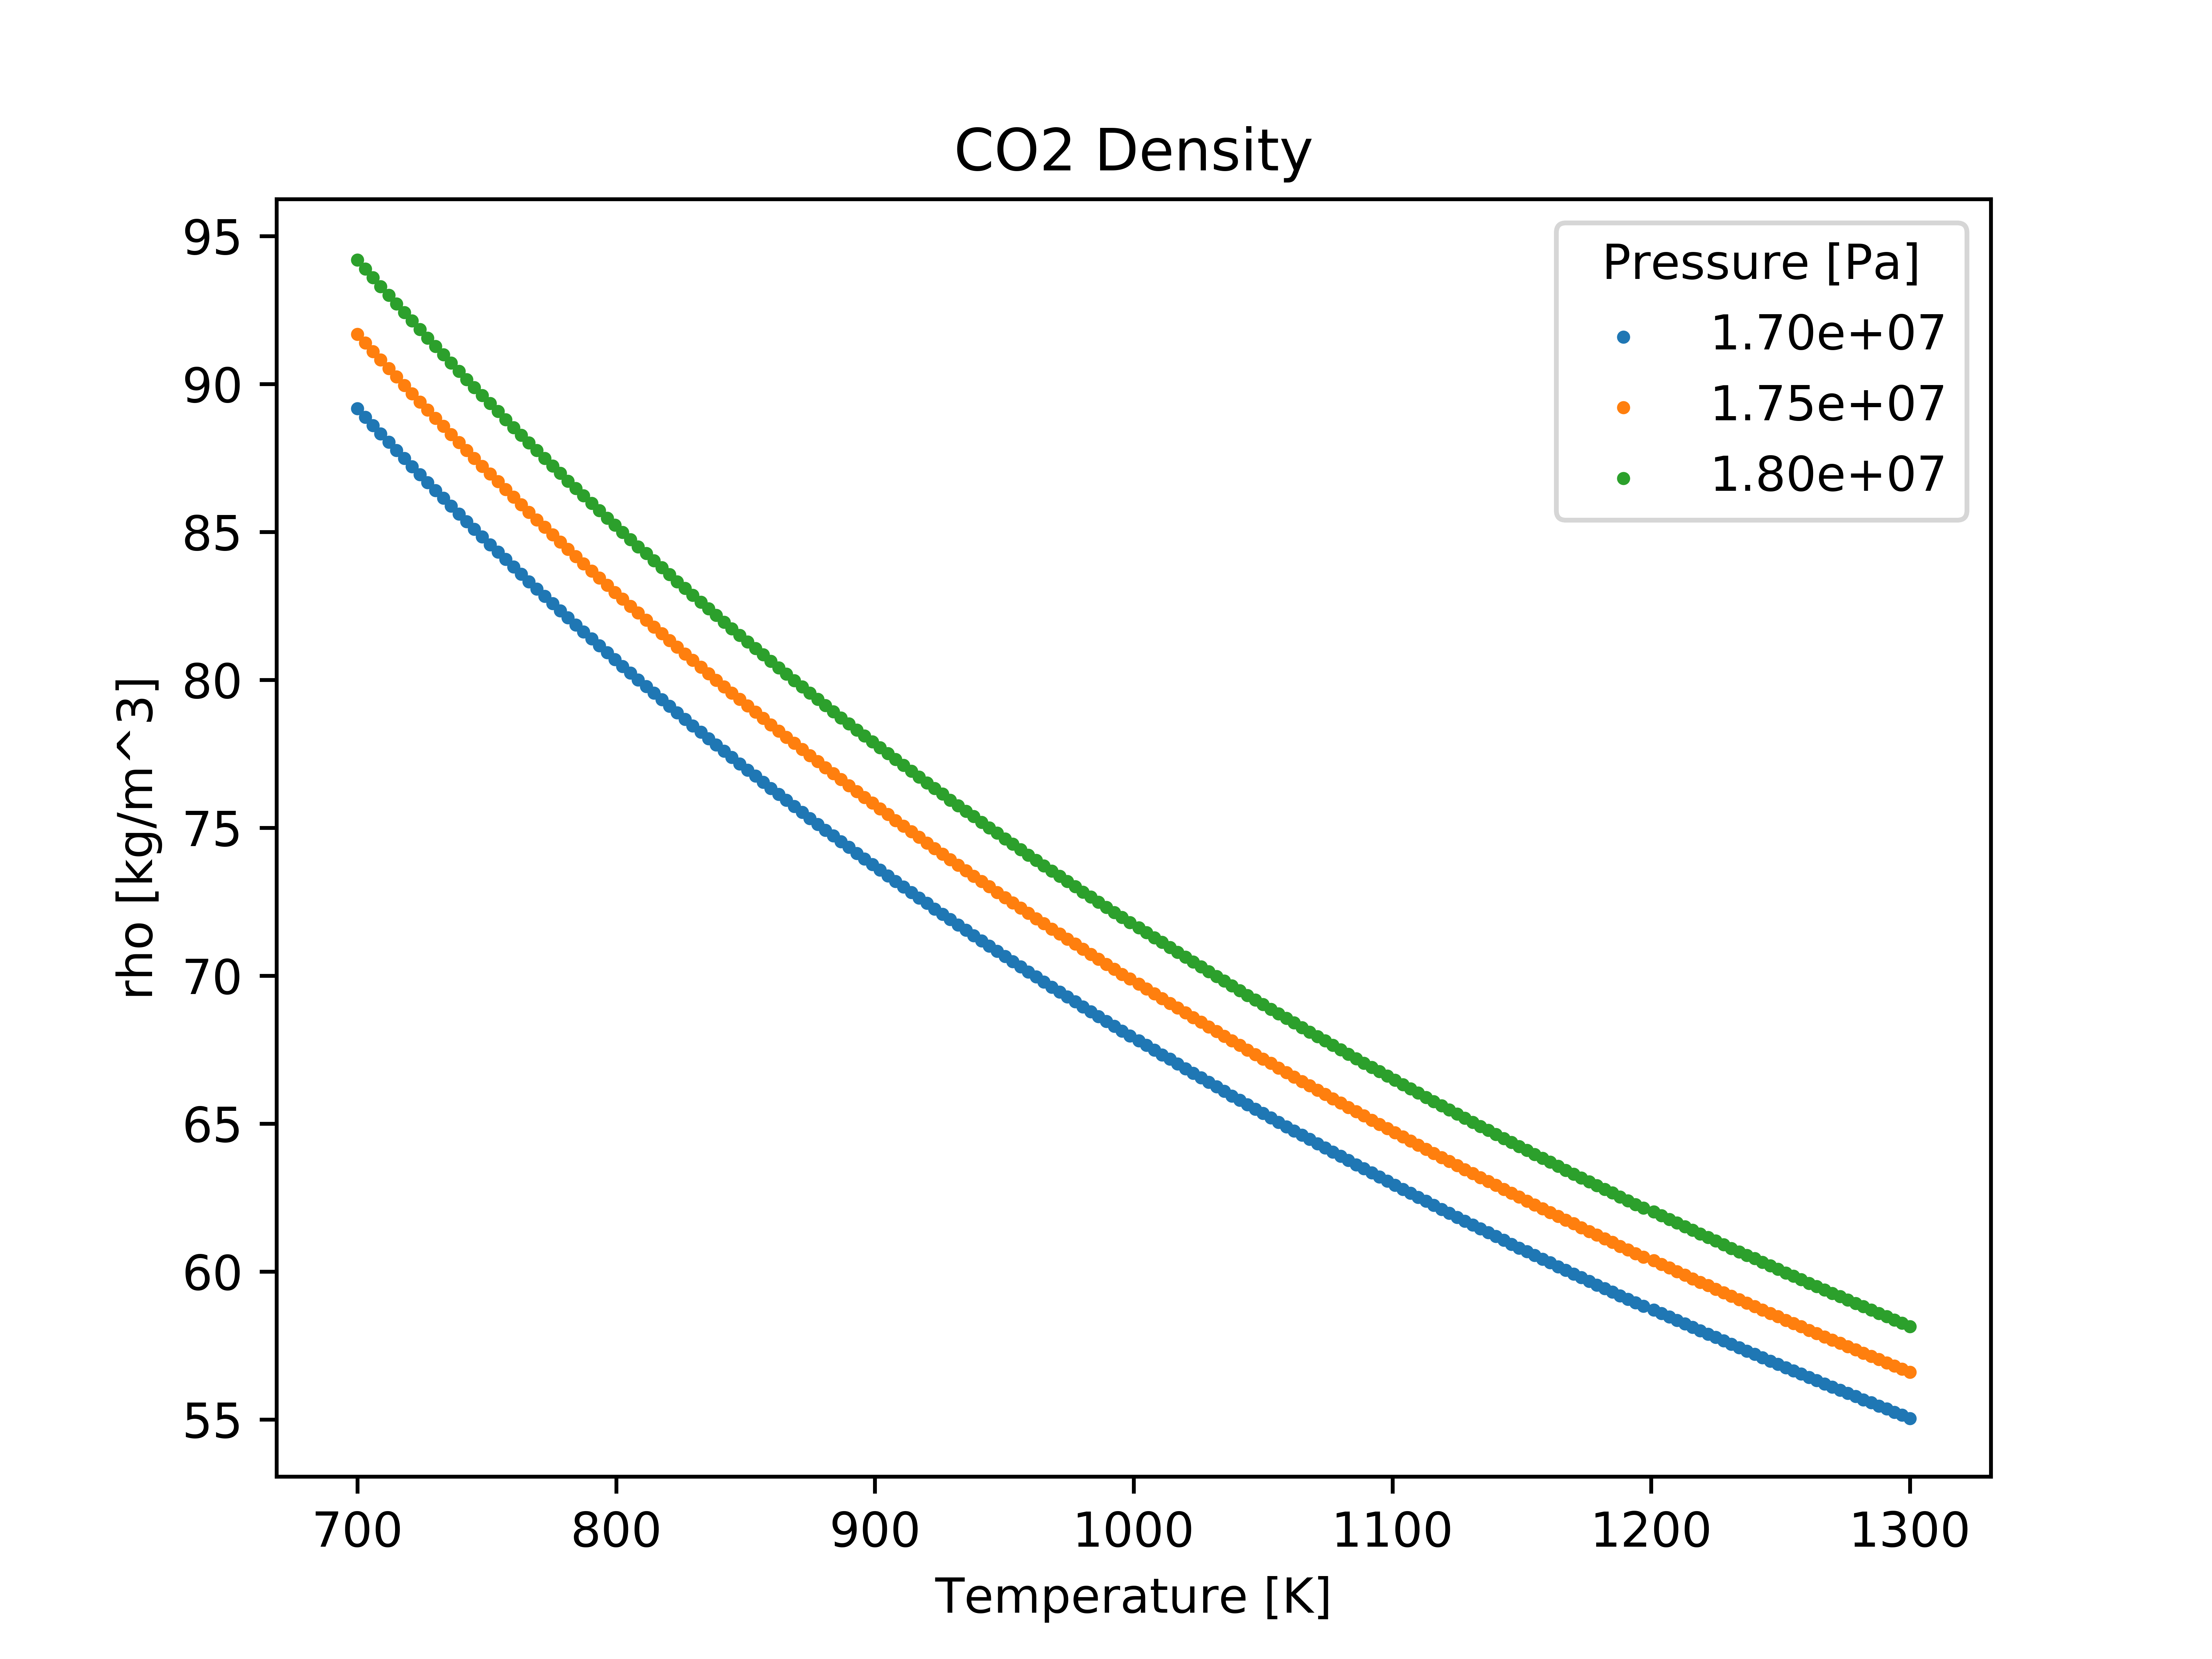
\includegraphics[width=4in]{../images/property_plots/CO2_Density.png}
\end{figure}

\begin{figure}[h]
    \centering
    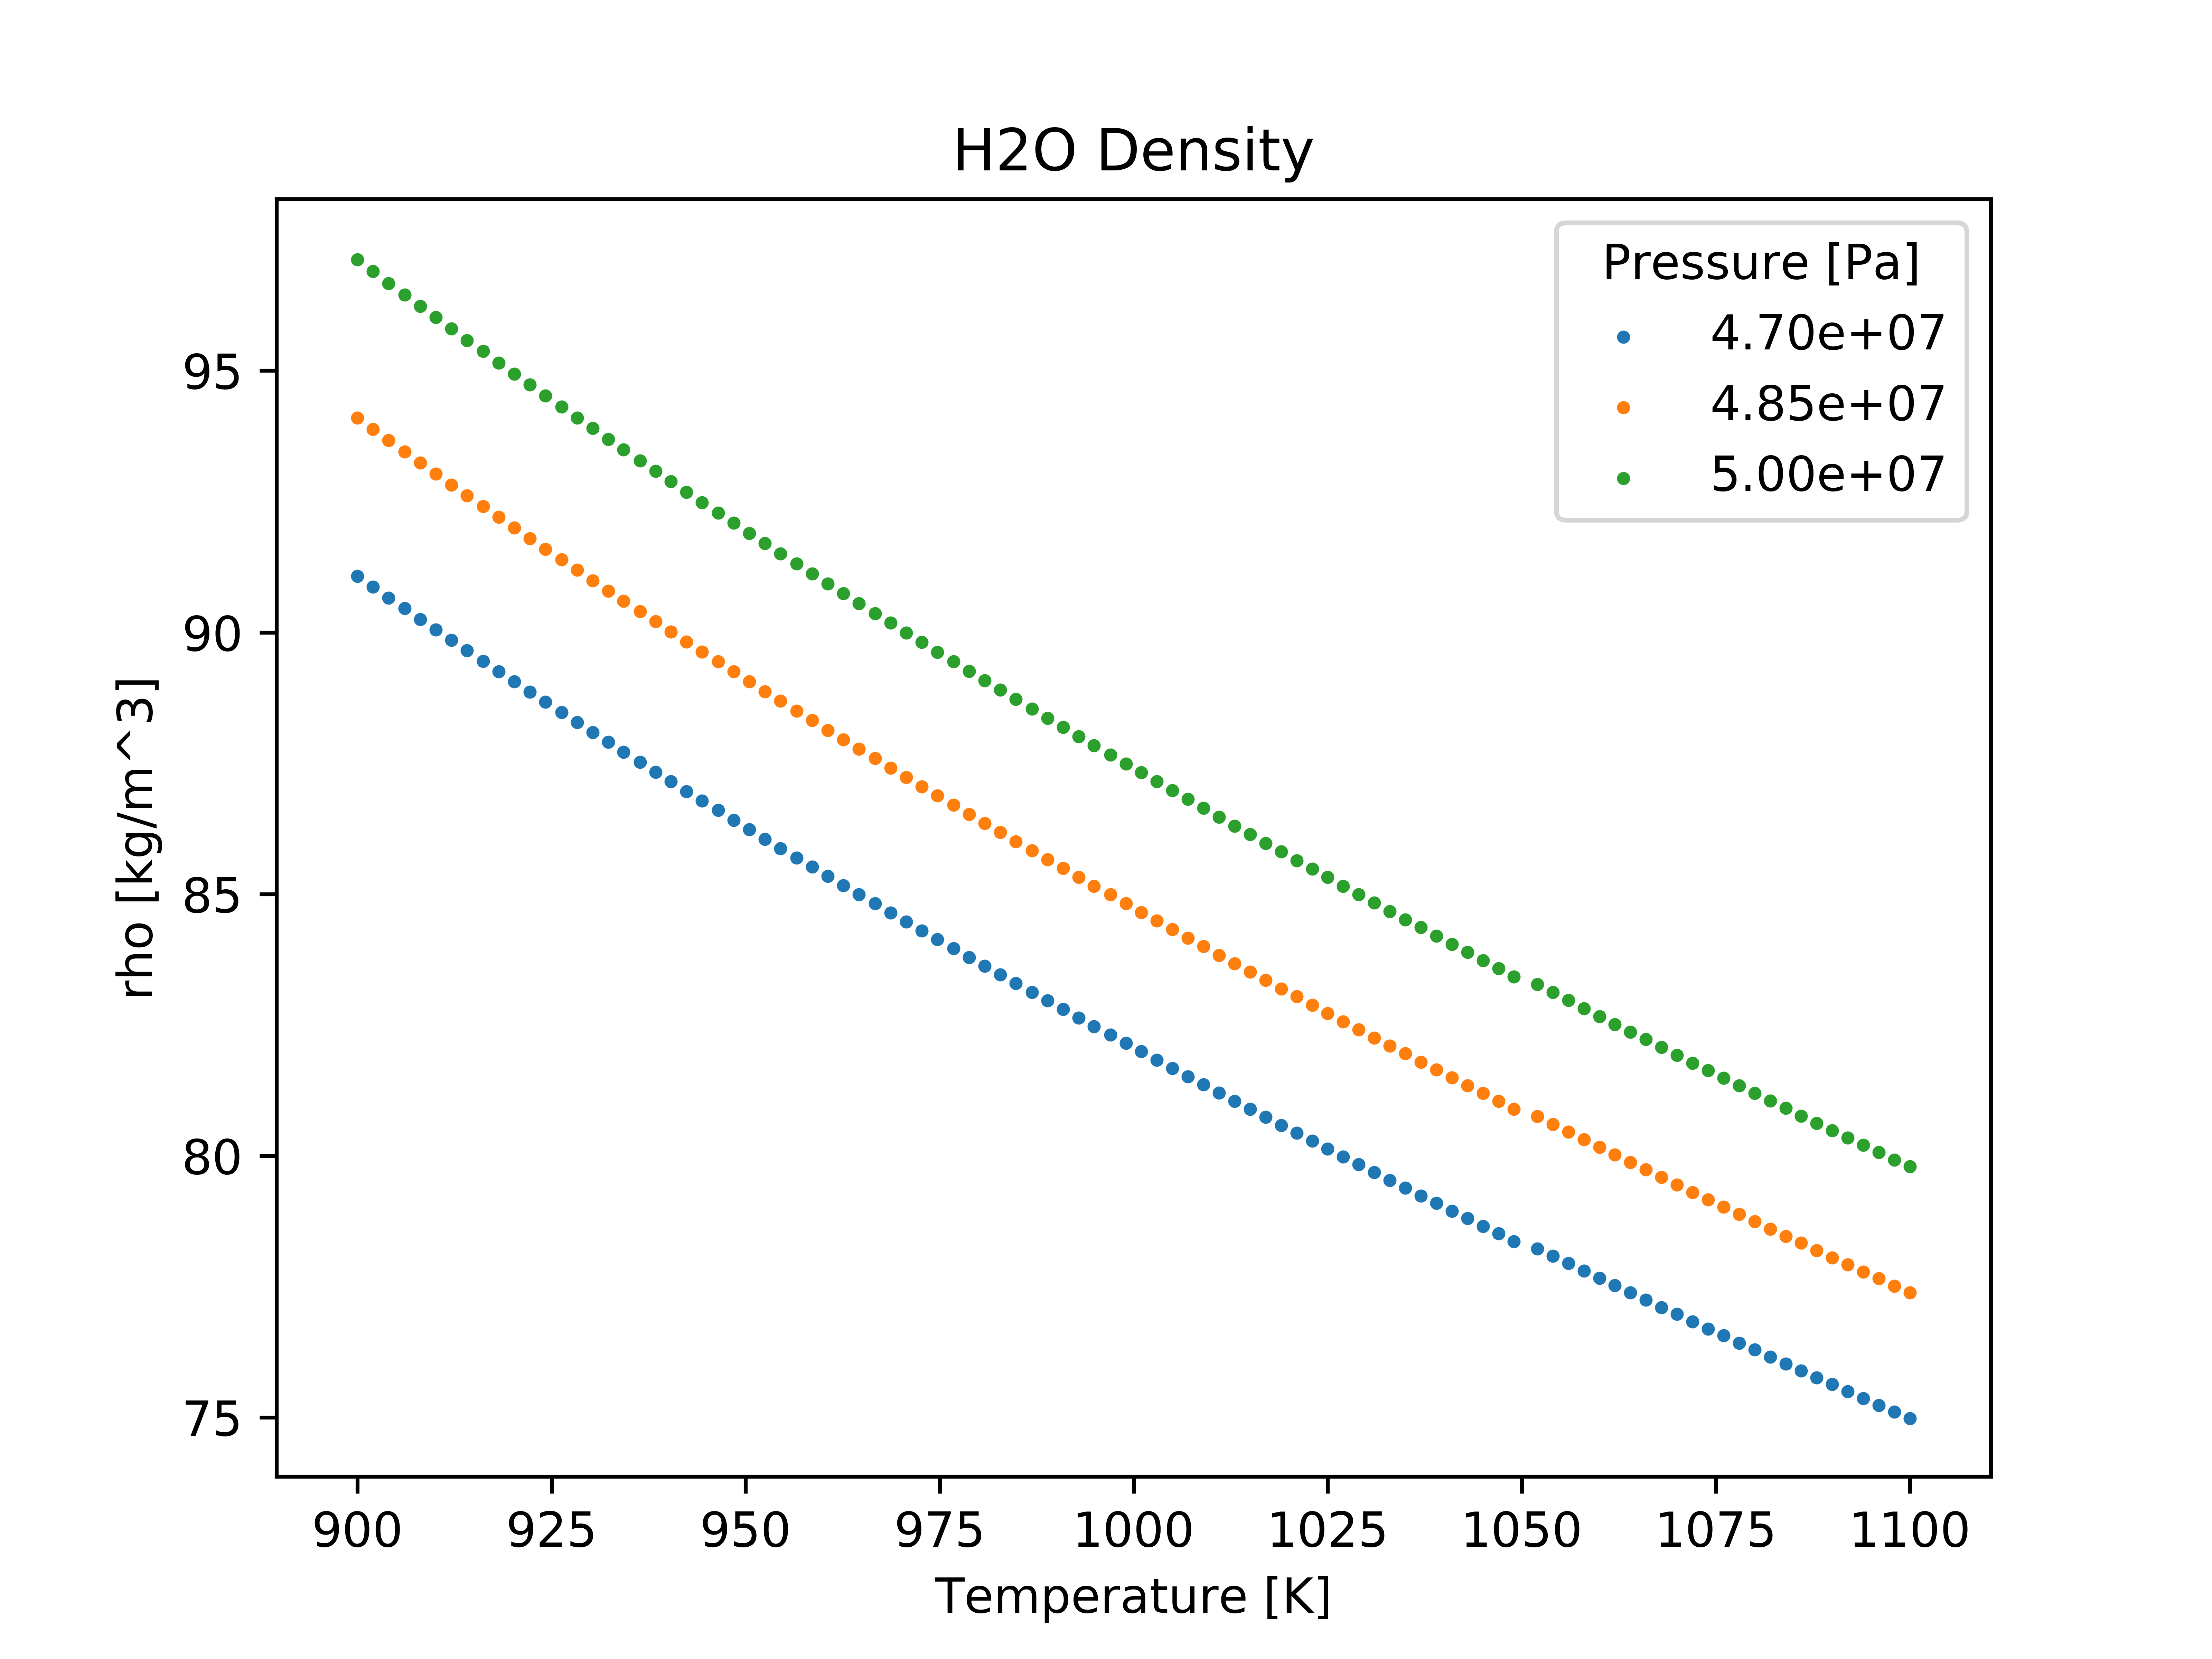
\includegraphics[width=4in]{../images/property_plots/H2O_Density.png}
\end{figure}

\begin{figure}[h]
    \centering
    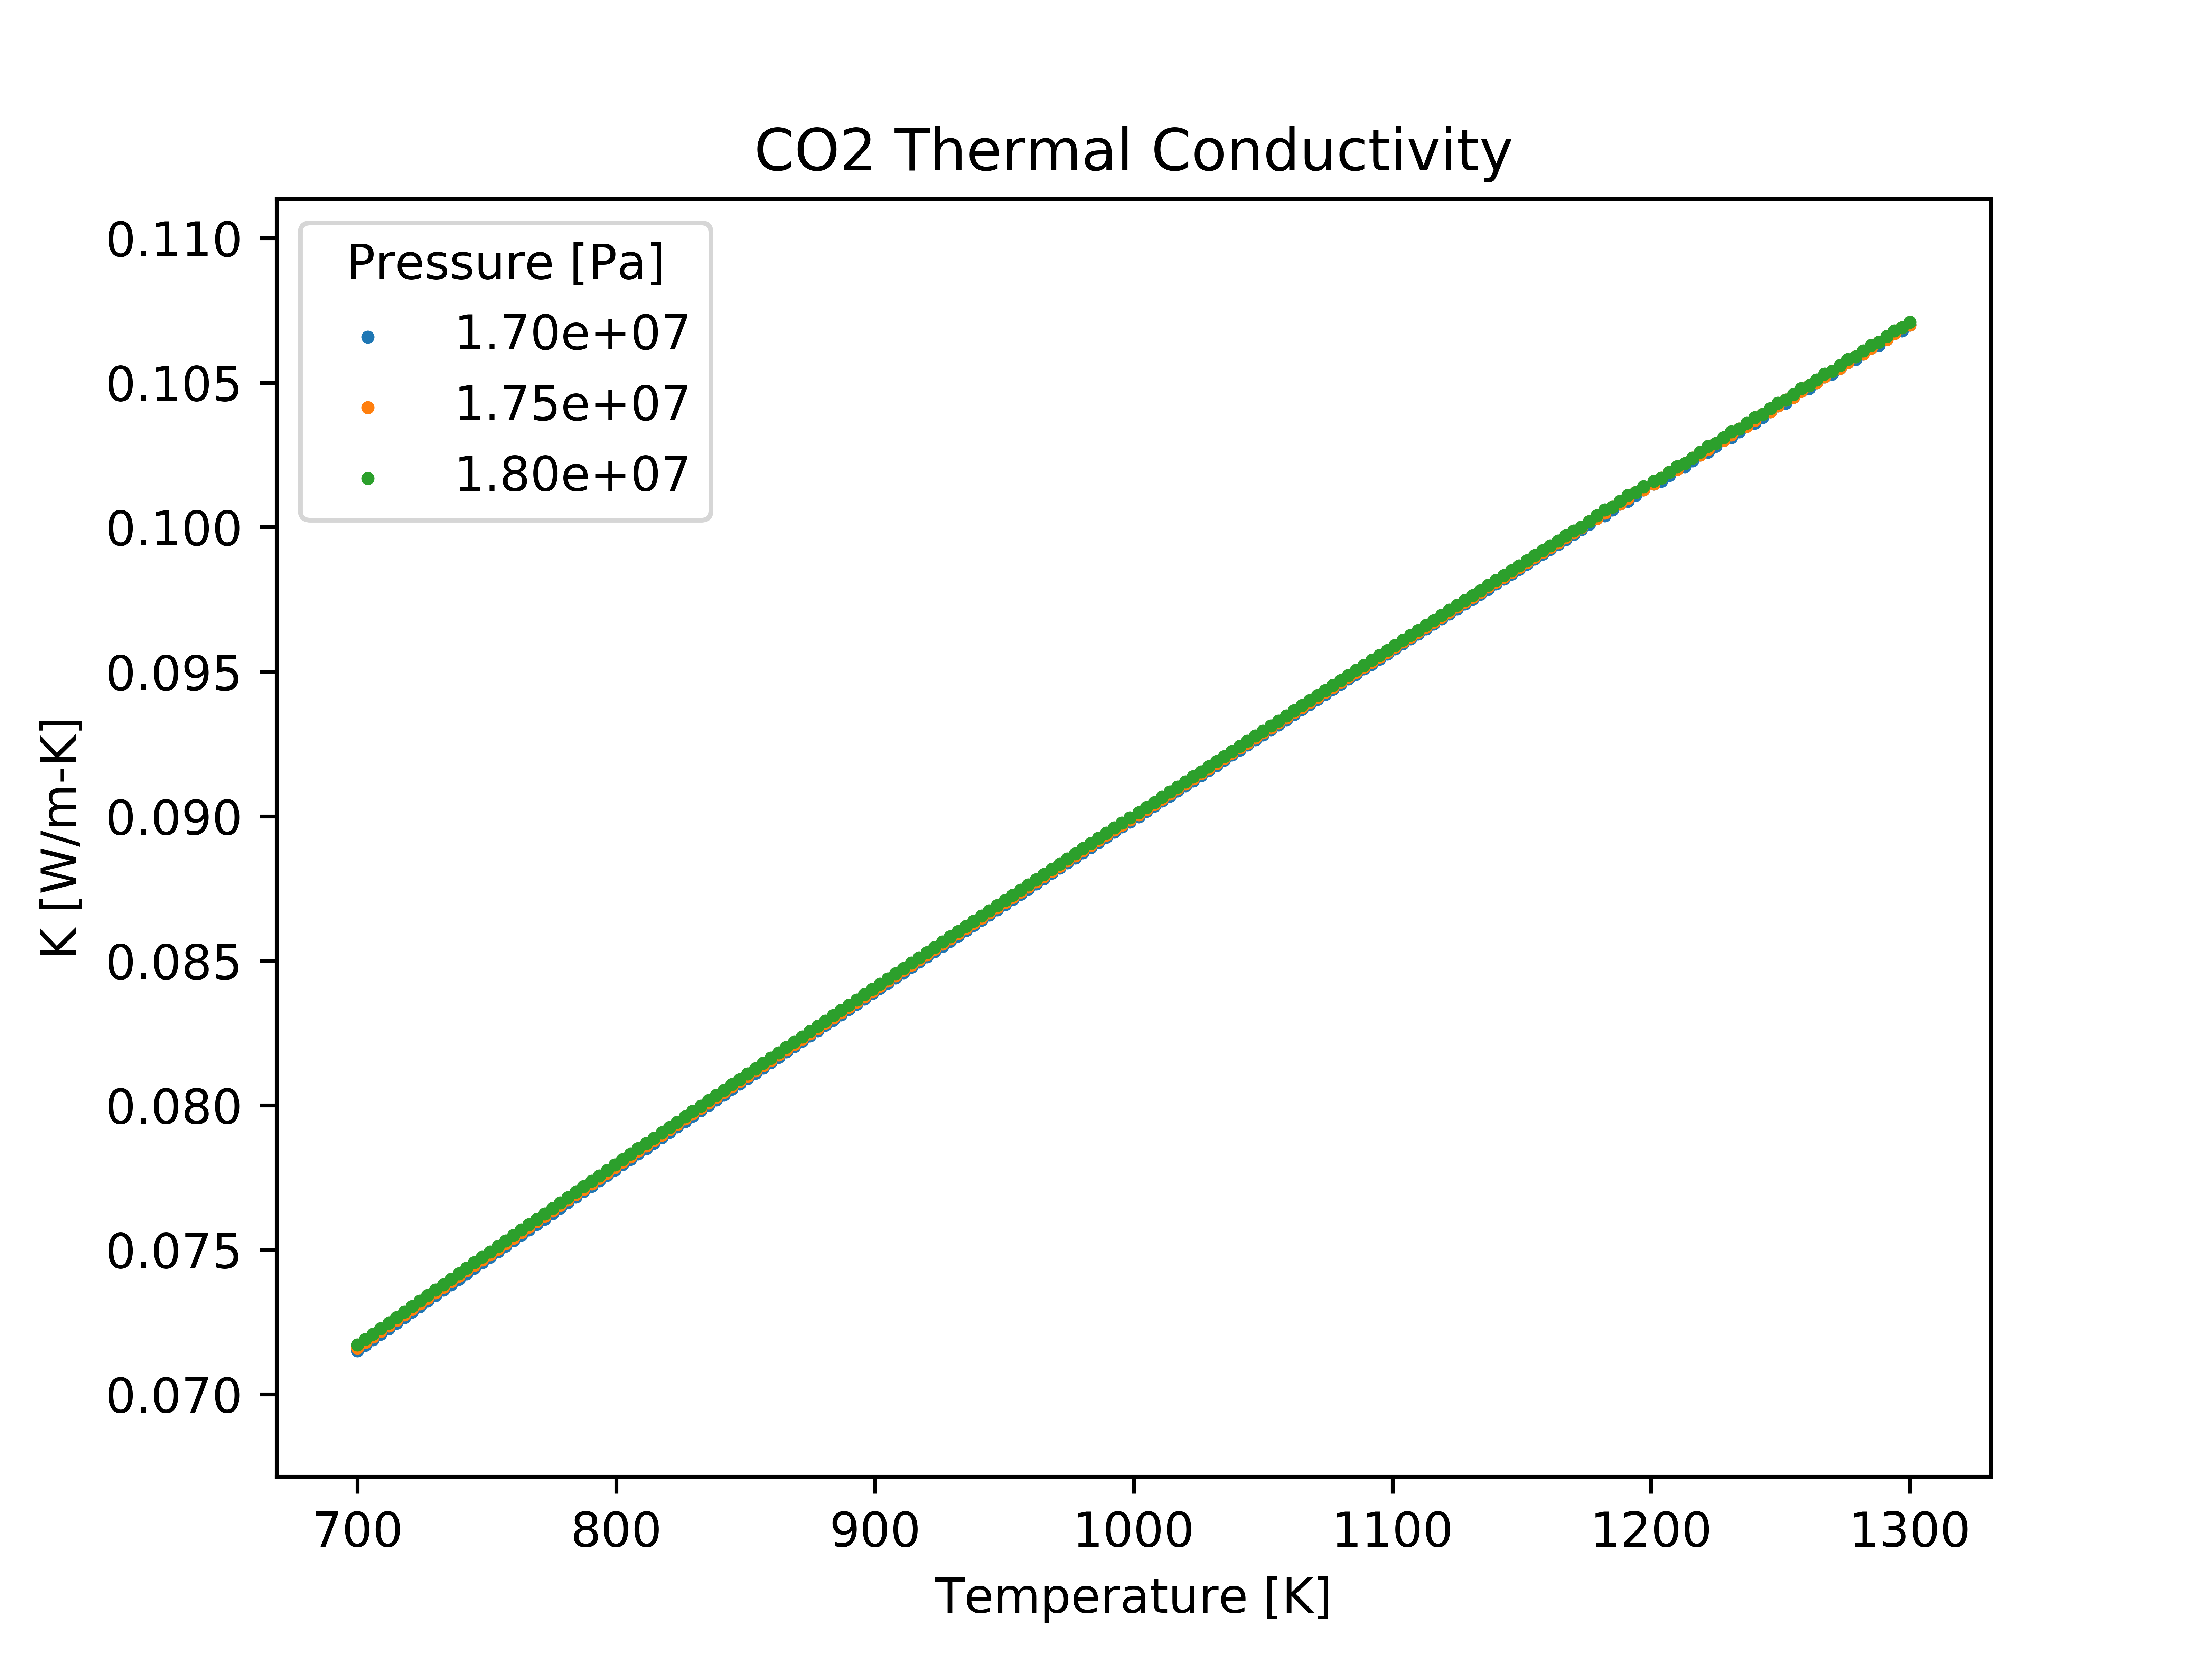
\includegraphics[width=4in]{../images/property_plots/CO2_Thermal_Conductivity.png}
\end{figure}

\begin{figure}[h]
    \centering
    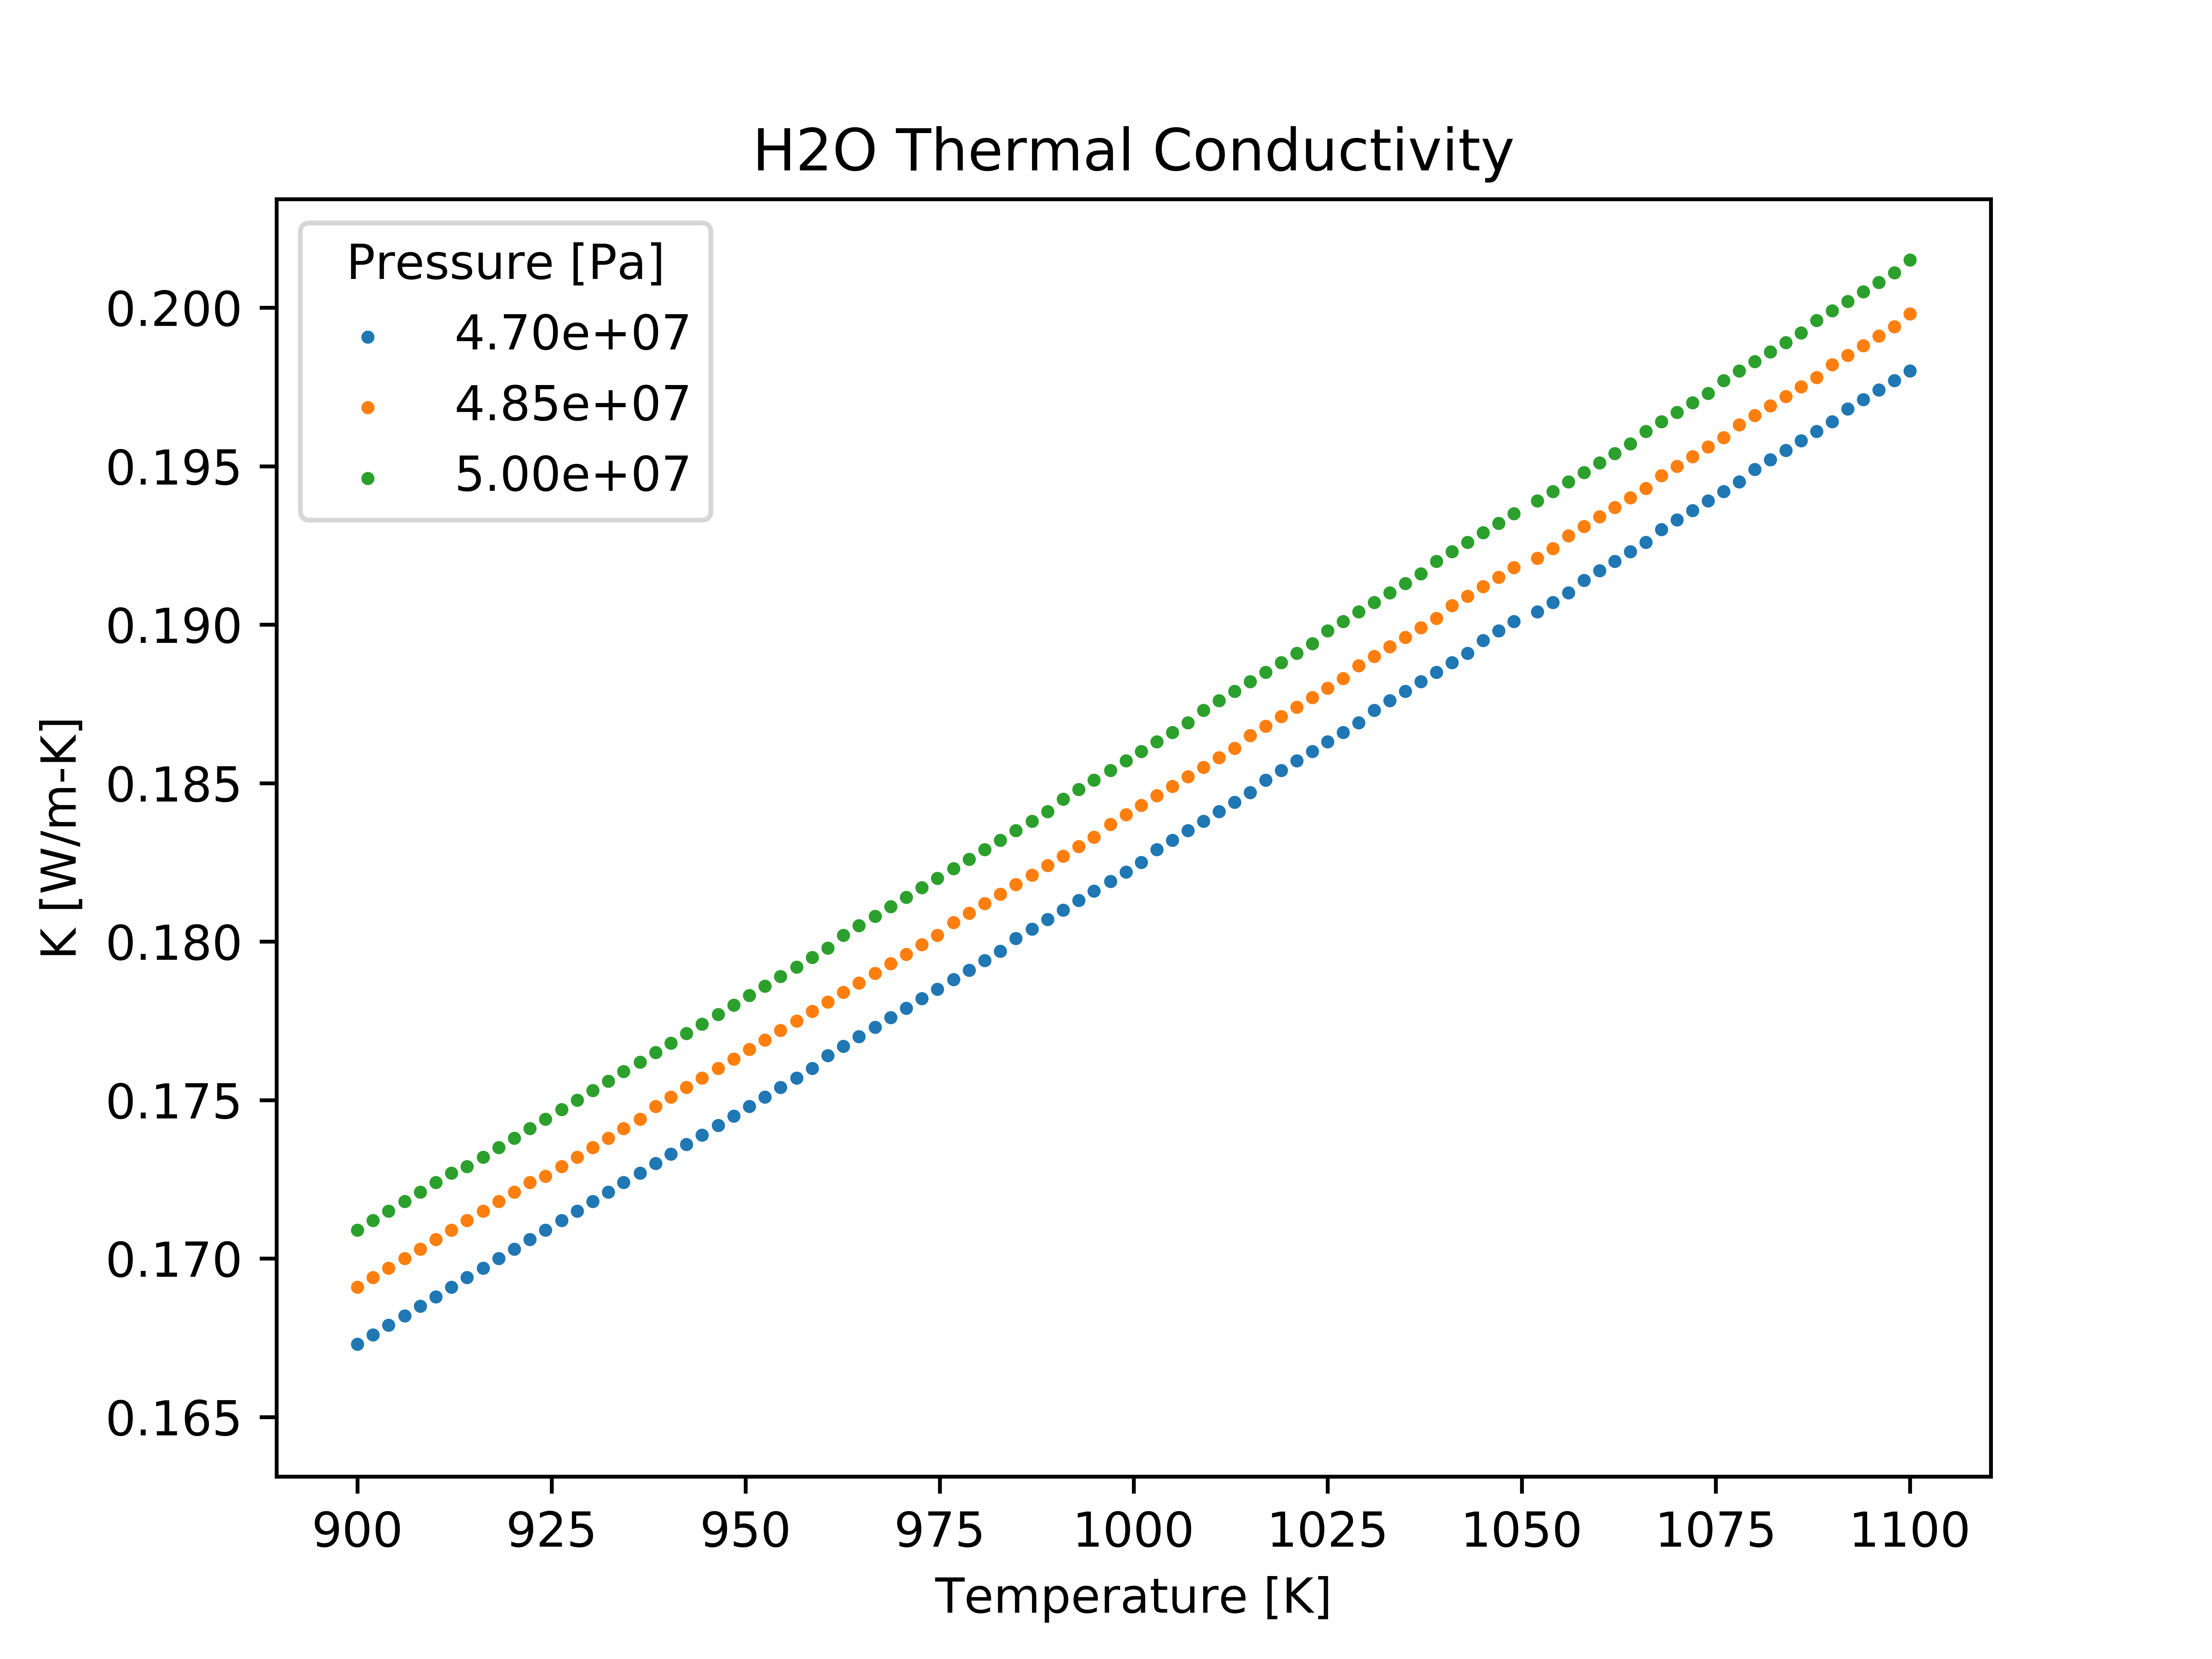
\includegraphics[width=4in]{../images/property_plots/H2O_Thermal_Conductivity.png}
\end{figure}

\begin{figure}[h]
    \centering
    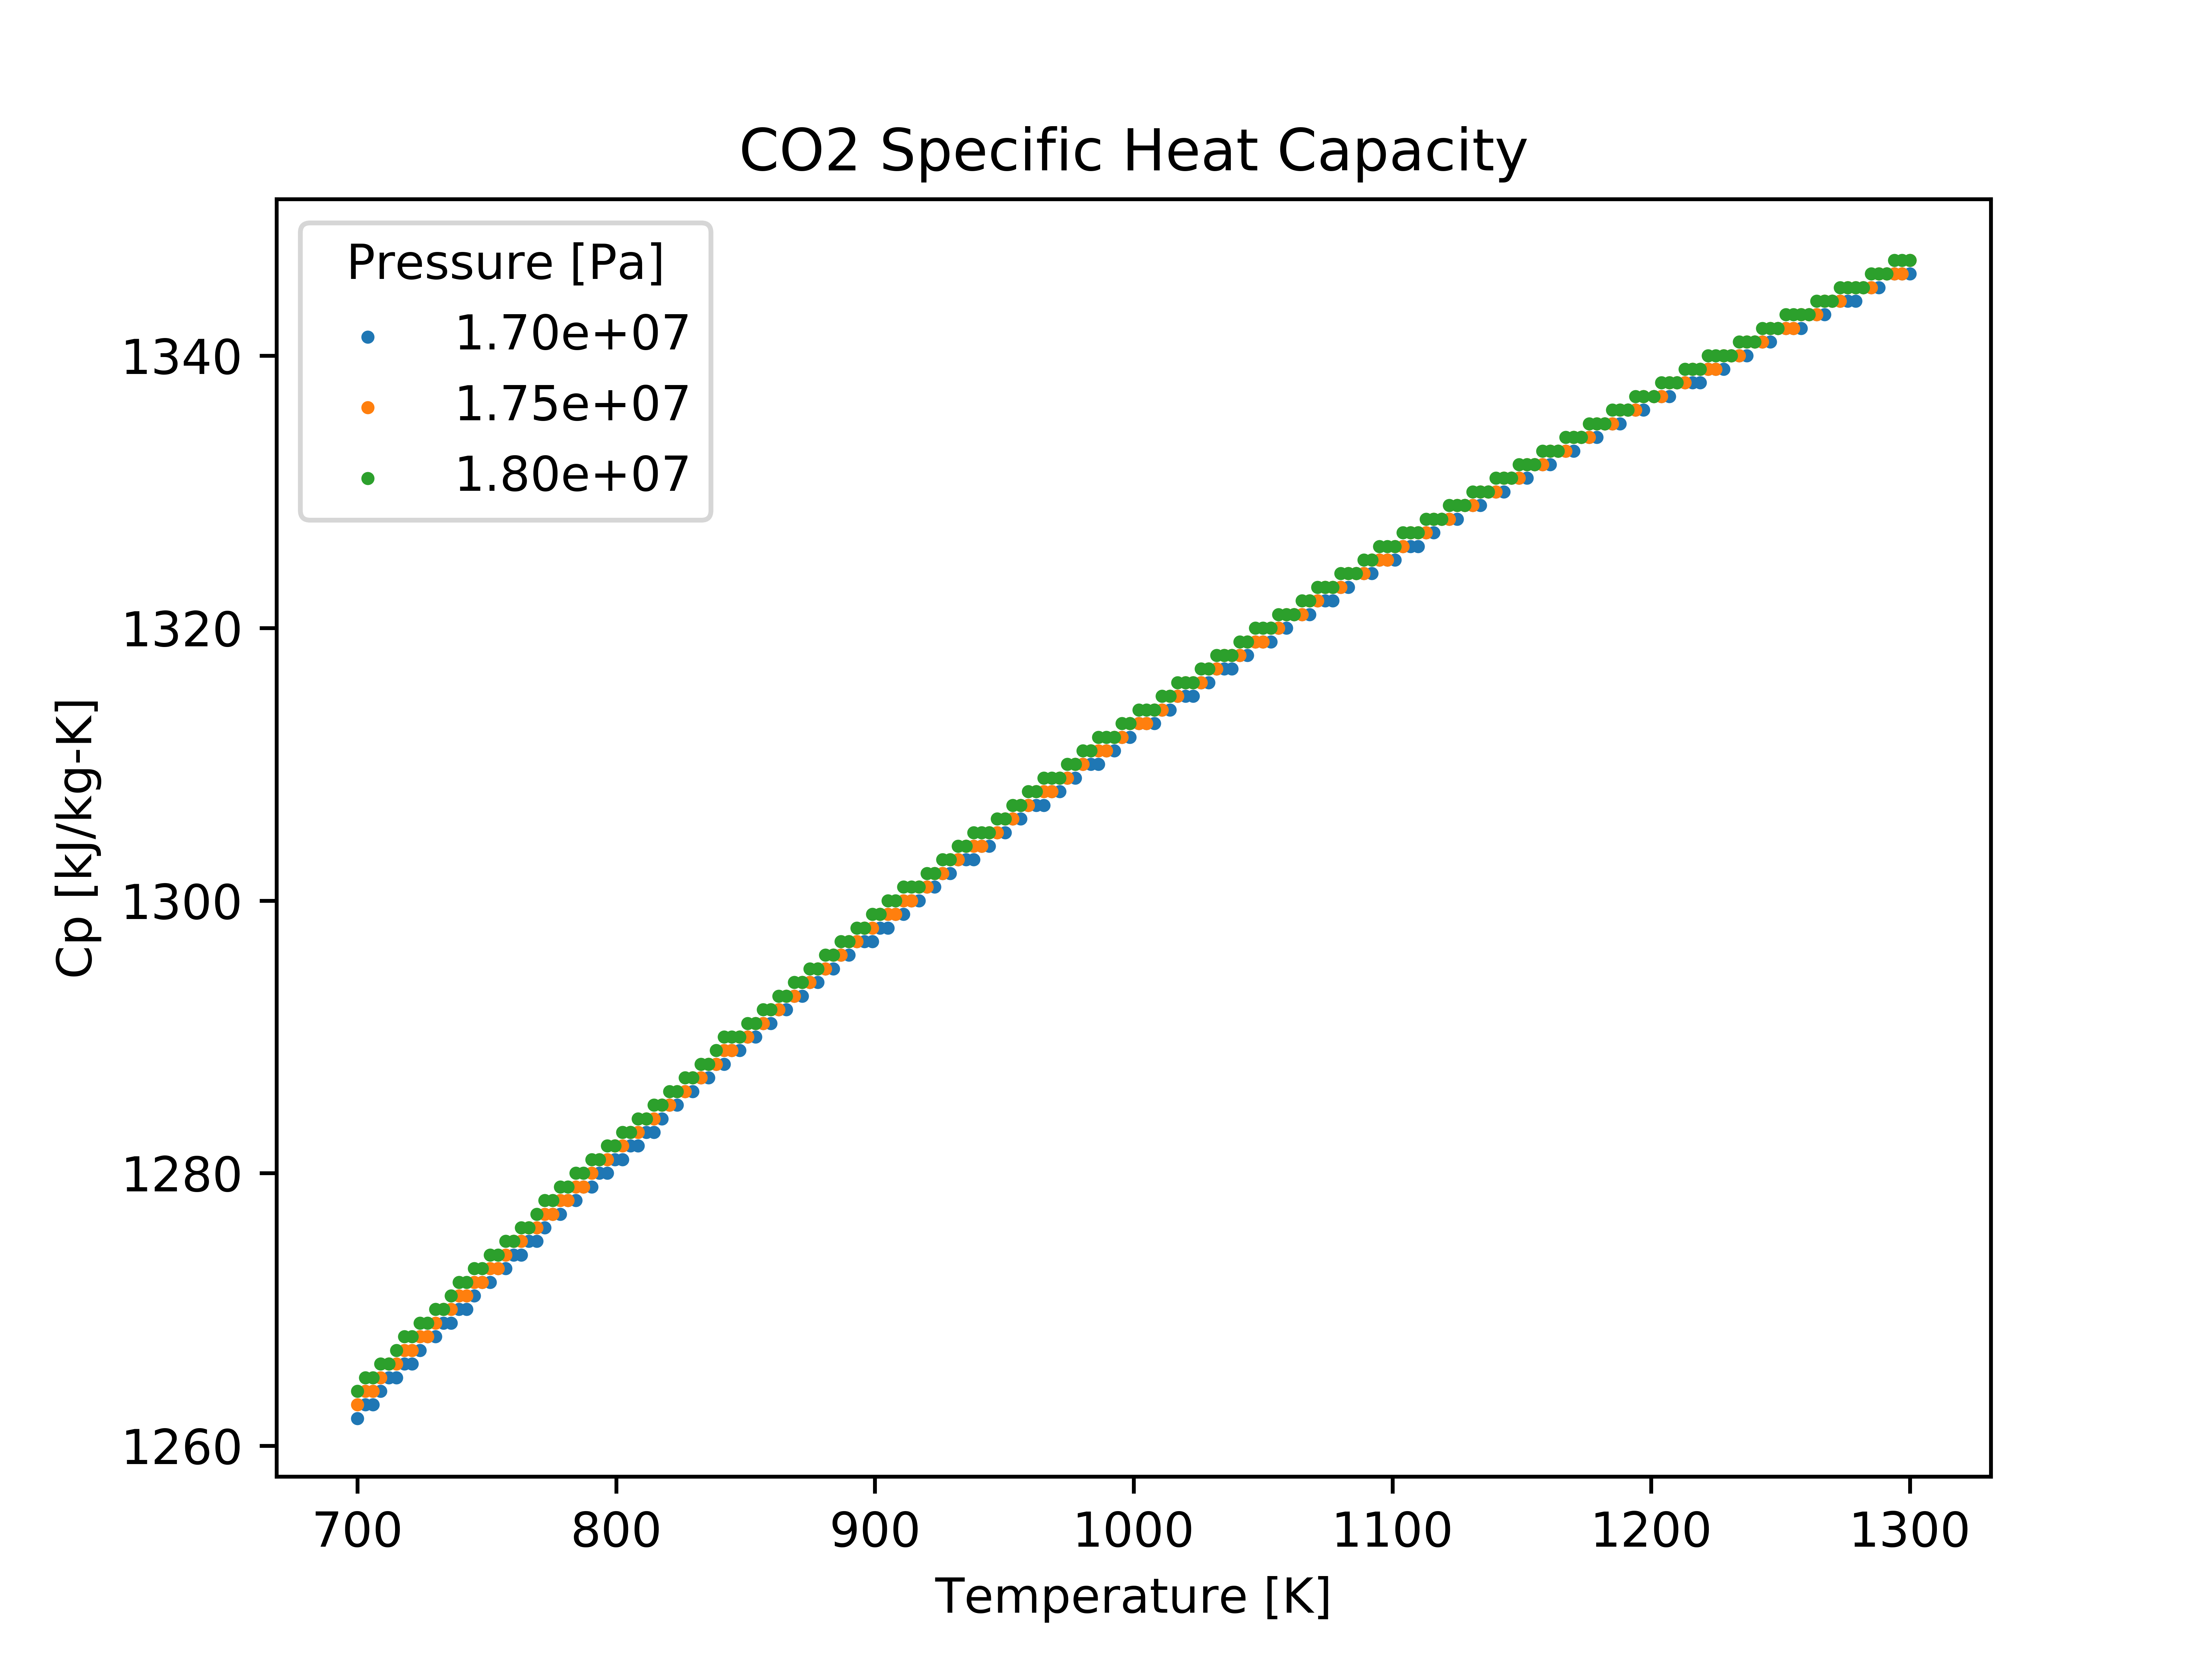
\includegraphics[width=4in]{../images/property_plots/CO2_Specific_Heat_Capacity.png}
\end{figure}

\begin{figure}[h]
    \centering
    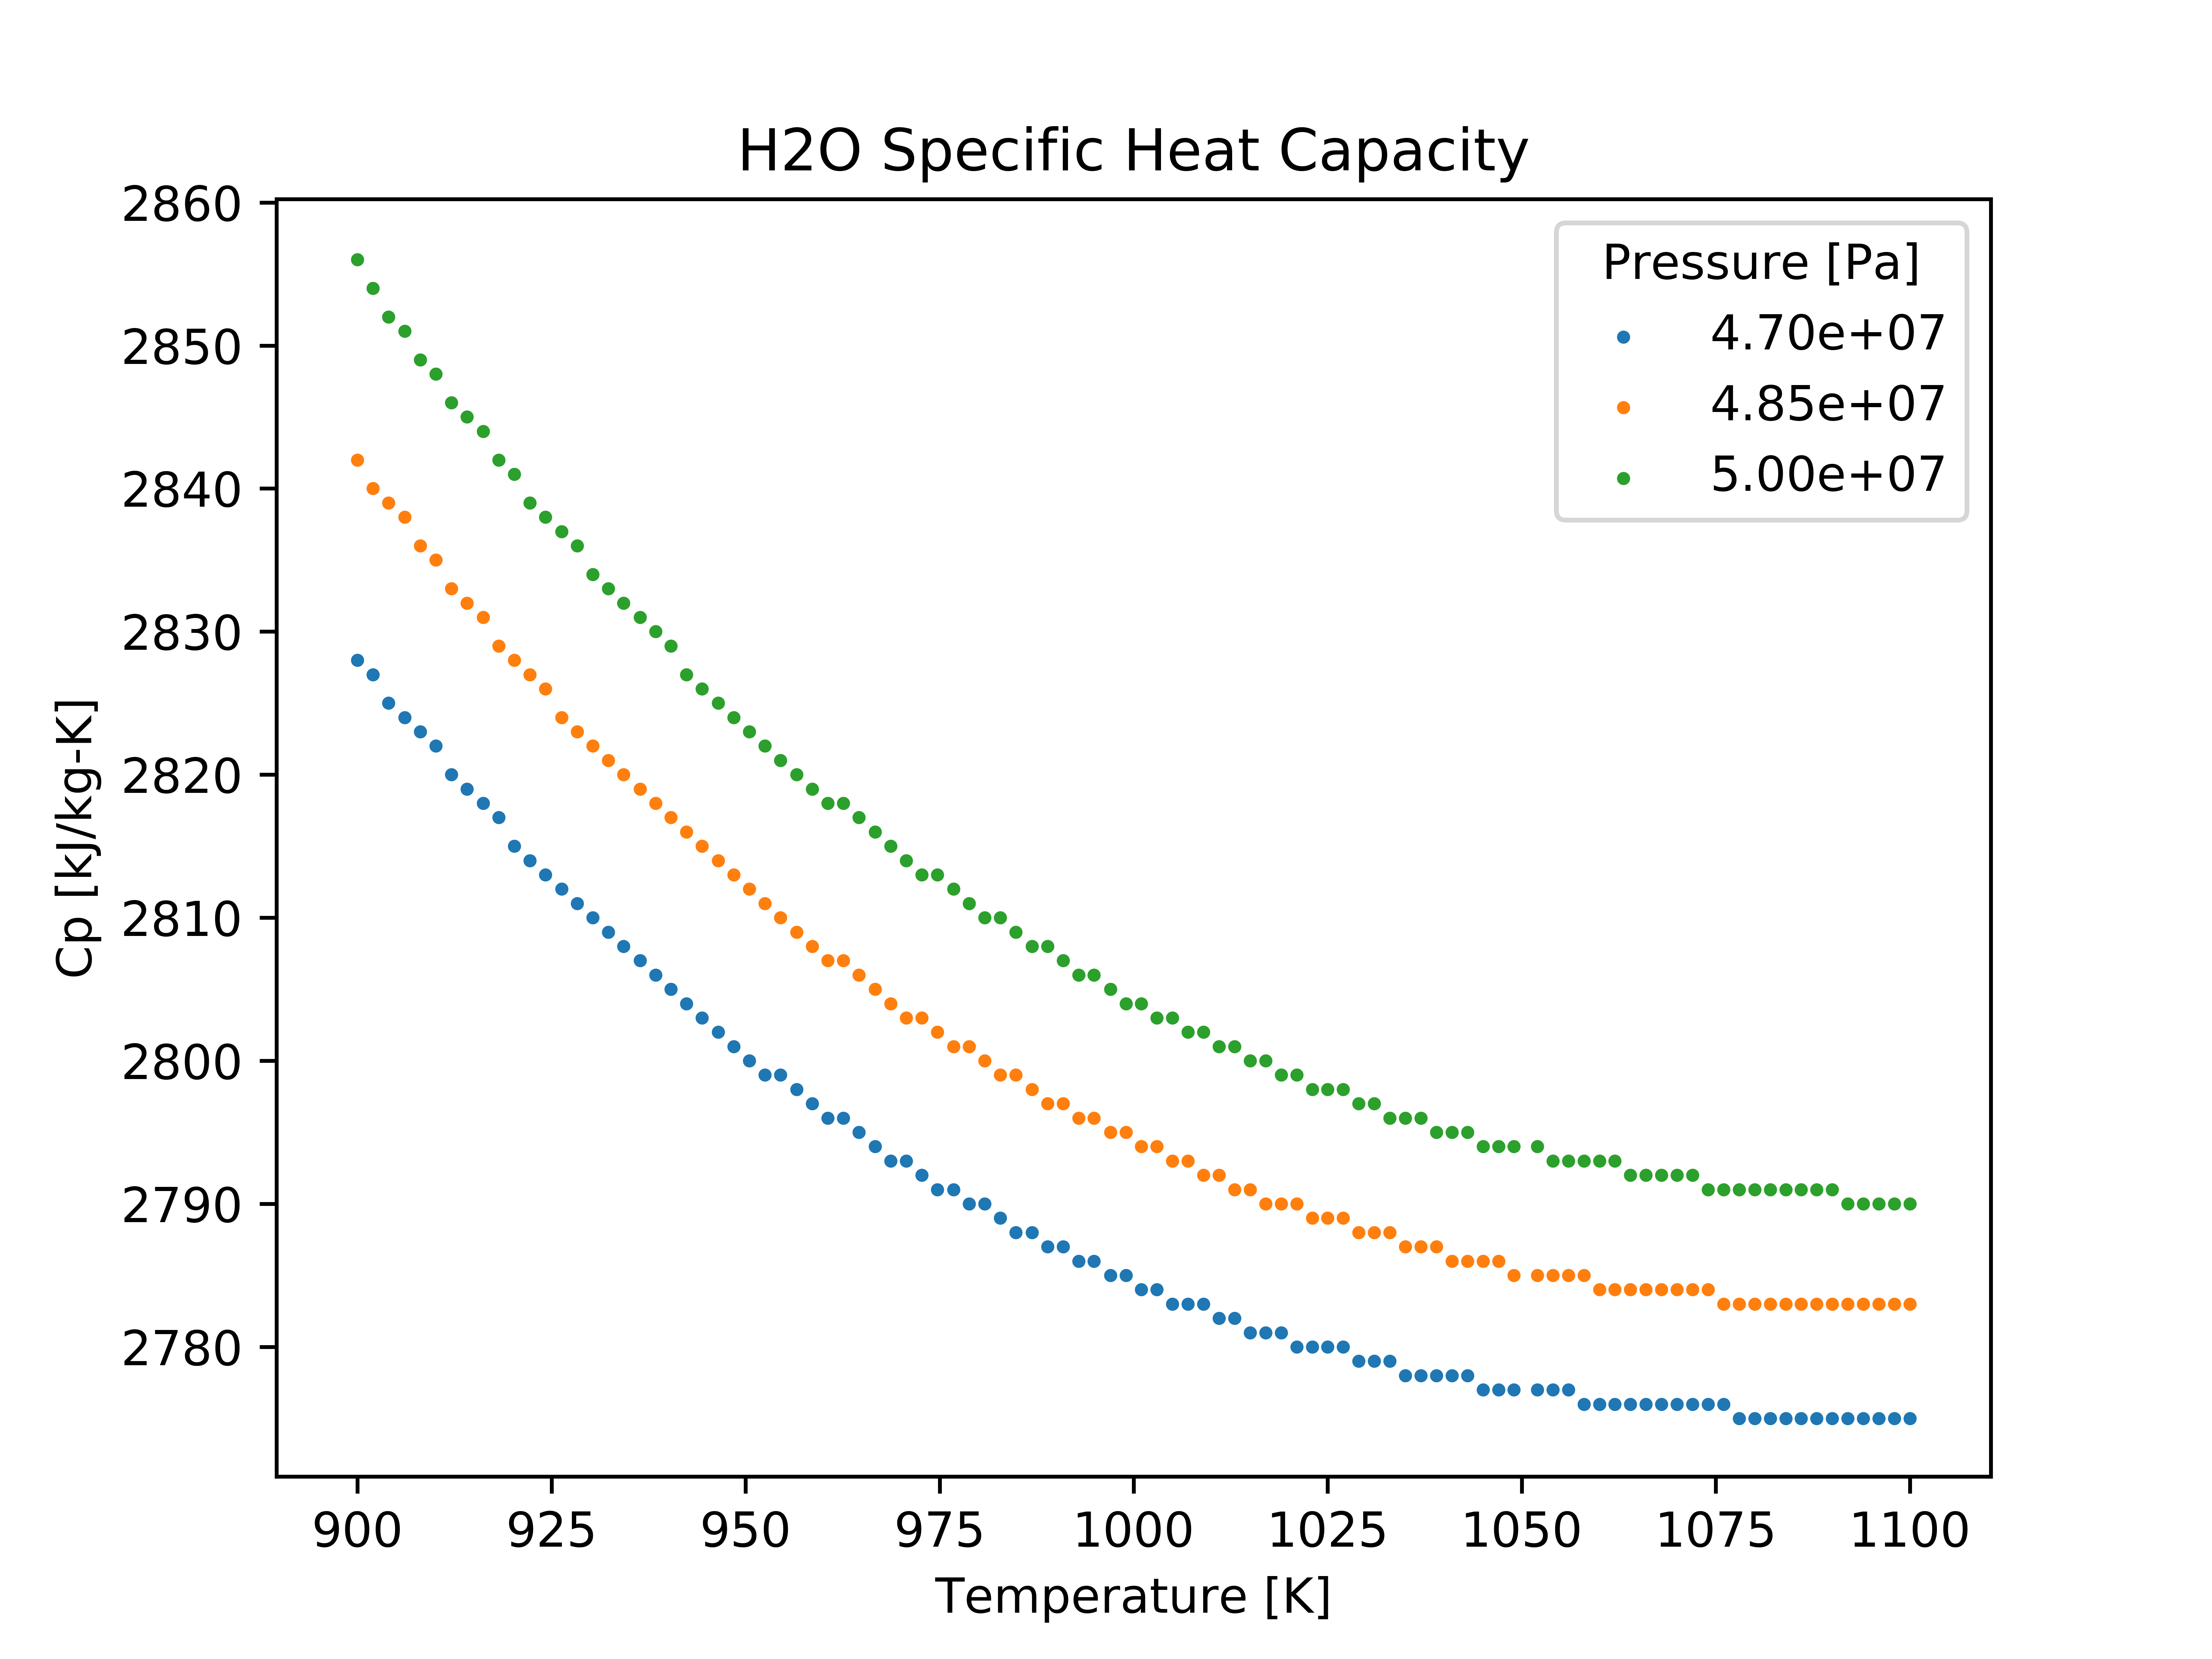
\includegraphics[width=4in]{../images/property_plots/H2O_Specific_Heat_Capacity.png}
\end{figure}

\begin{figure}[h]
    \centering
    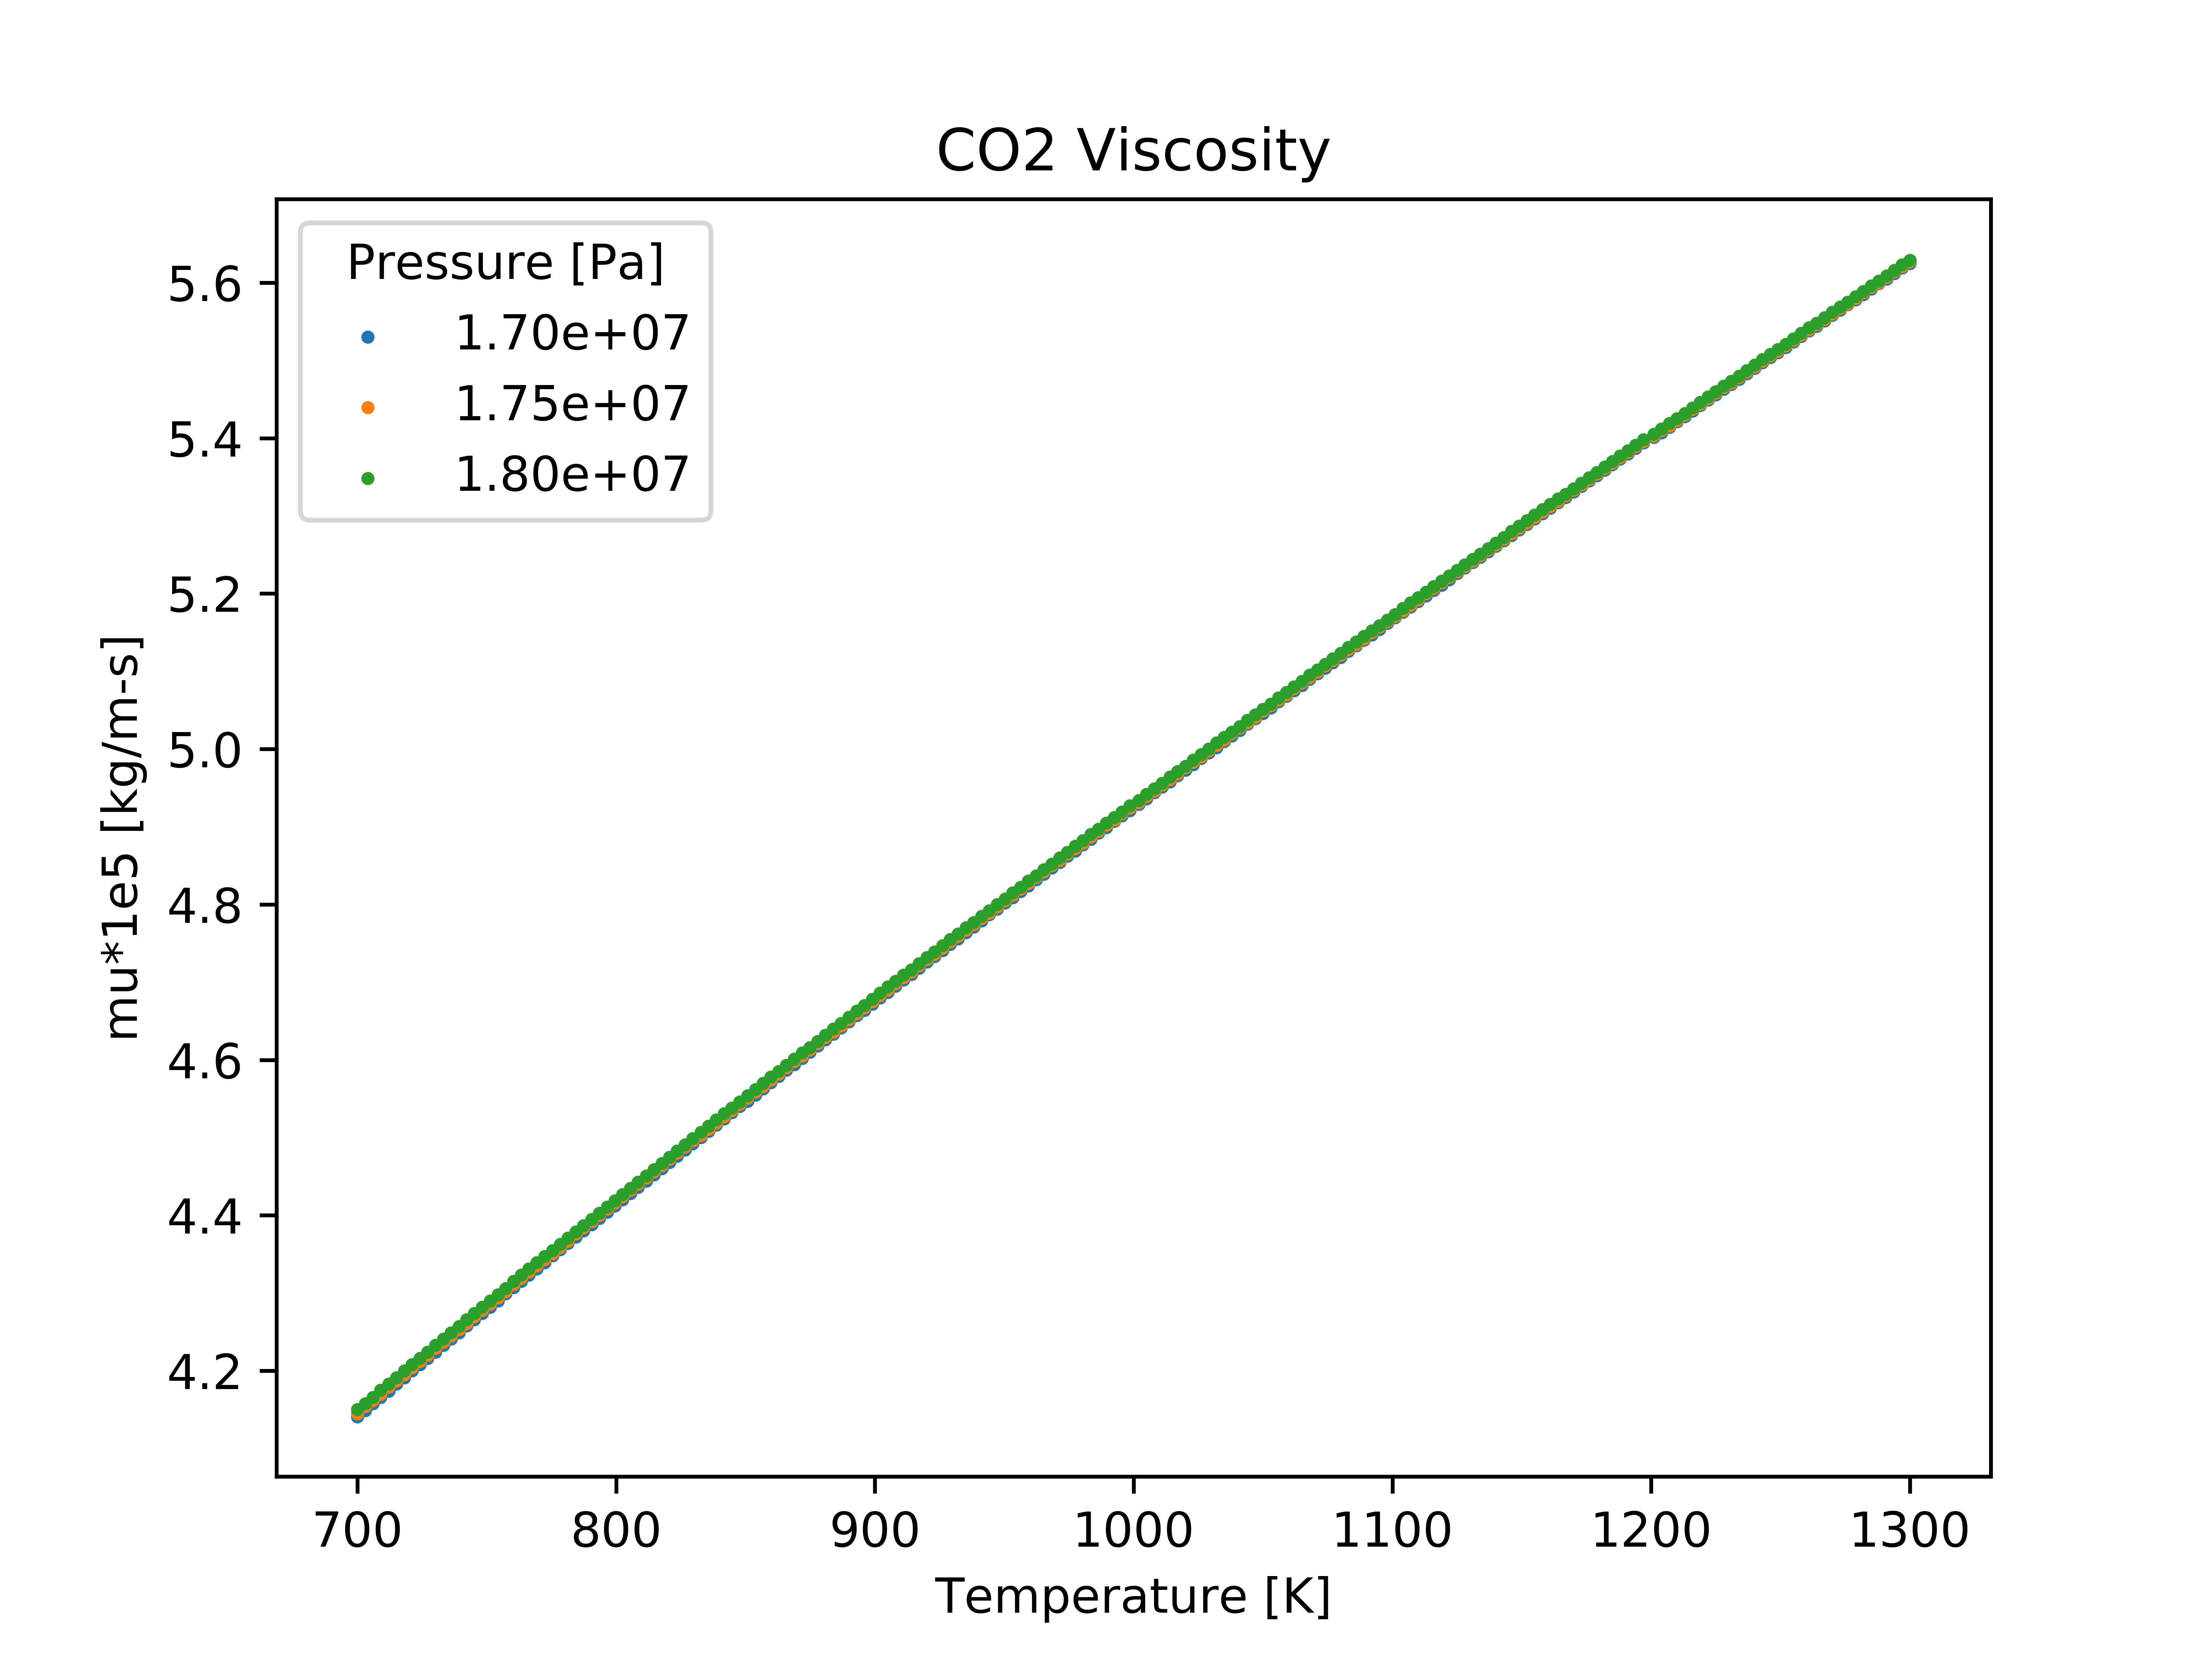
\includegraphics[width=4in]{../images/property_plots/CO2_Viscosity.png}
\end{figure}

\begin{figure}[h]
    \centering
    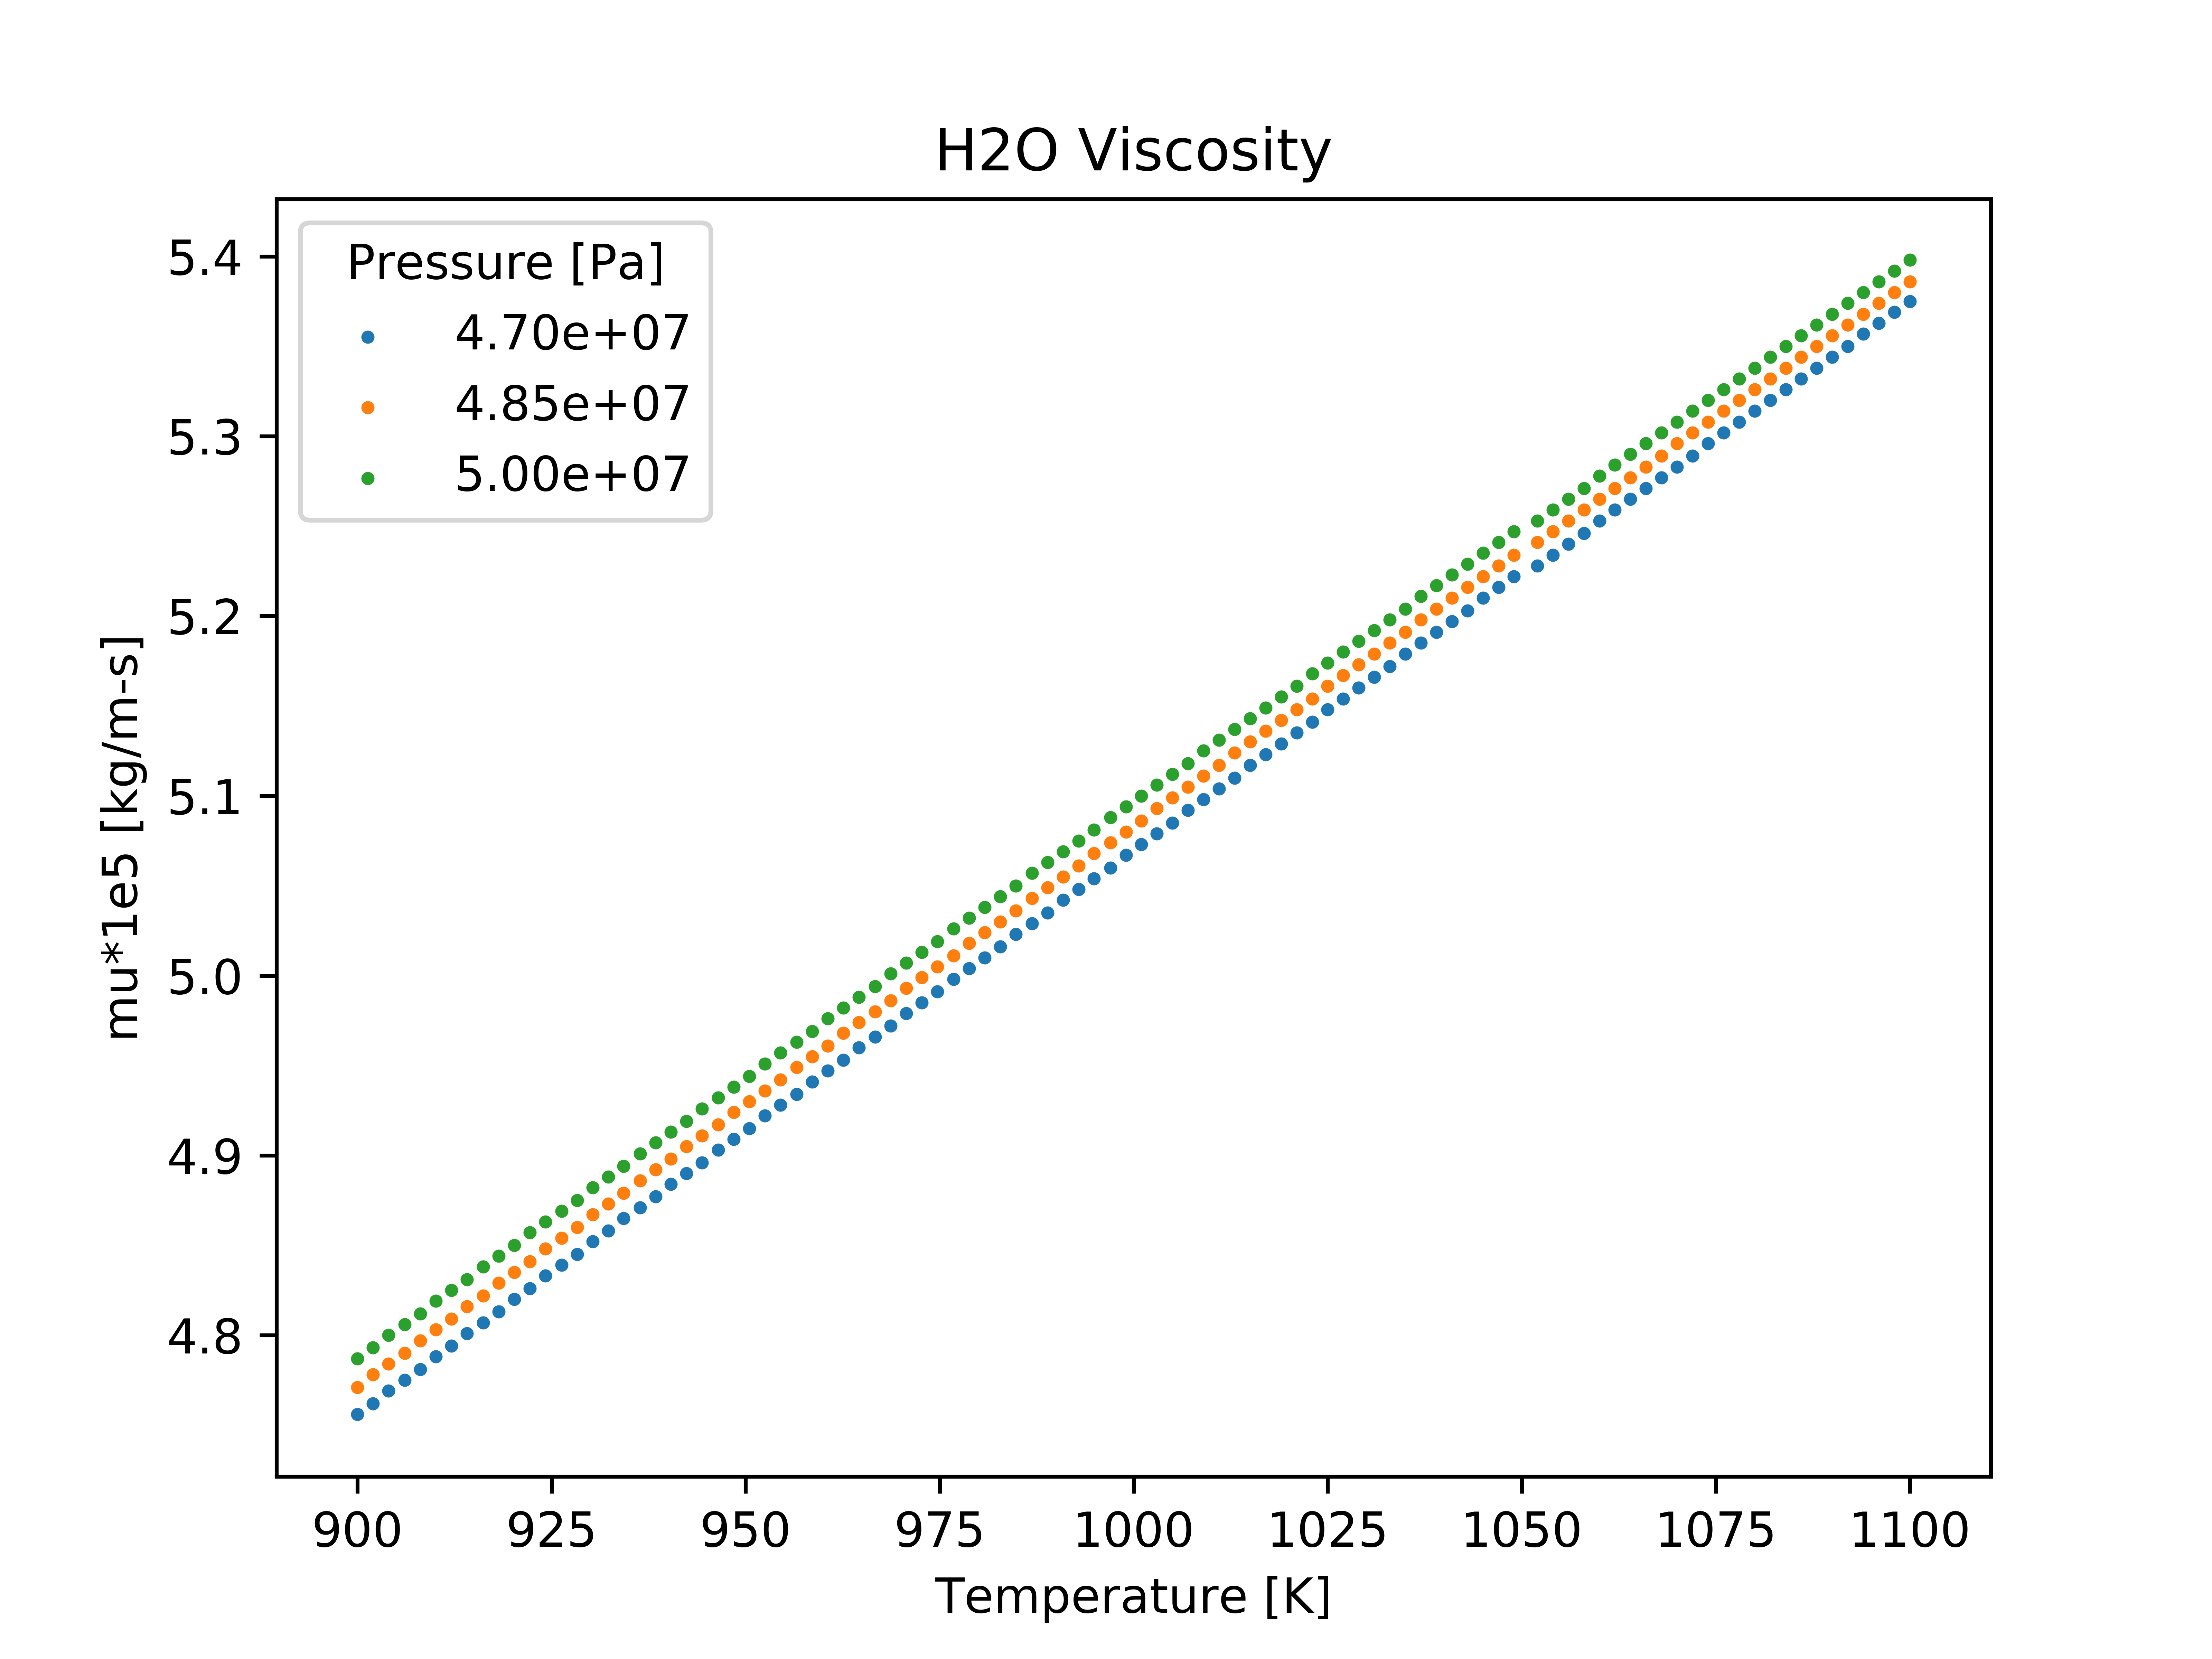
\includegraphics[width=4in]{../images/property_plots/H2O_Viscosity.png}
\end{figure}
